
% ----------------------------------------------------------------------
%  Set the document class
% ----------------------------------------------------------------------
\documentclass[11pt,a4paper,twoside]{article}

% ----------------------------------------------------------------------
% Define external packages, language, margins, fonts and new commands
% ----------------------------------------------------------------------
%\input{preamble} 
\usepackage[utf8]{inputenc}   % <<<<< Linux
\usepackage[english]{babel} % <<<<< English
\usepackage{notoccite}
\usepackage[skip=0.5\baselineskip]{caption}
\hyphenation{GTKWave}
\usepackage{ragged2e}
\usepackage{tabto}
\usepackage{listings}
\usepackage[all]{nowidow}

%blind text
\usepackage{lipsum}

\usepackage{graphicx}
\graphicspath{ {./} {../../figlib/} }
\def\FontLn{% 16 pt normal
  \usefont{T1}{phv}{m}{n}\fontsize{16pt}{16pt}\selectfont}
\def\FontLb{% 16 pt bold
  \usefont{T1}{phv}{b}{n}\fontsize{16pt}{16pt}\selectfont}
\def\FontMn{% 14 pt normal
  \usefont{T1}{phv}{m}{n}\fontsize{14pt}{14pt}\selectfont}
\def\FontMb{% 14 pt bold
  \usefont{T1}{phv}{b}{n}\fontsize{14pt}{14pt}\selectfont}
\def\FontSn{% 12 pt normal
  \usefont{T1}{phv}{m}{n}\fontsize{12pt}{12pt}\selectfont}

% Use Arial font as default
%
\renewcommand{\rmdefault}{phv}
\renewcommand{\sfdefault}{phv}
\usepackage{geometry}	
\geometry{verbose,tmargin=2.5cm,bmargin=2.5cm,lmargin=2.5cm,rmargin=2.5cm}

%\usepackage{setspace}
%\renewcommand{\baselinestretch}{1.5}

\usepackage[pdftex]{hyperref} % enhance documents that are to be
                              % output as HTML and PDF
\hypersetup{colorlinks,       % color text of links and anchors,
                              % eliminates borders around links
%            linkcolor=red,    % color for normal internal links
            linkcolor=black,  % color for normal internal links
            anchorcolor=black,% color for anchor text
%            citecolor=green,  % color for bibliographical citations
            citecolor=black,  % color for bibliographical citations
%            filecolor=magenta,% color for URLs which open local files
            filecolor=black,  % color for URLs which open local files
%            menucolor=red,    % color for Acrobat menu items
            menucolor=black,  % color for Acrobat menu items
%            pagecolor=red,    % color for links to other pages
            pagecolor=black,  % color for links to other pages
%            urlcolor=cyan,    % color for linked URLs
            urlcolor=black,   % color for linked URLs
	          bookmarks=true,         % create PDF bookmarks
	          bookmarksopen=false,    % don't expand bookmarks
	          bookmarksnumbered=true, % number bookmarks
	          pdftitle={report},
            pdfauthor={Andre C. Marta},
%            pdfsubject={Thesis Title},
%            pdfkeywords={Thesis Keywords},
            pdfstartview=FitV,
            pdfdisplaydoctitle=true}

\usepackage[numbers,sort&compress]{natbib} % <<<<< References in numbered list [1],[2],...
\usepackage{subcaption} 
\usepackage{mdframed}

%%%%%%%%%%%%%%%%%%%%%%%%%%%%%%%%%%%%%%%%%%%%%%%%%%%%%%%%%%%%%%%%%%%%%%%%
%     Begin Document                                                   %
%%%%%%%%%%%%%%%%%%%%%%%%%%%%%%%%%%%%%%%%%%%%%%%%%%%%%%%%%%%%%%%%%%%%%%%%


\begin{document}

% Set plain page style (no headers, footer with centered page number)
\pagestyle{plain}

% Set roman numbering (i,ii,...) before the start of chapters
%\pagenumbering{roman}

% ----------------------------------------------------------------------
%  Cover page
% ----------------------------------------------------------------------
%%%%%%%%%%%%%%%%%%%%%%%%%%%%%%%%%%%%%%%%%%%%%%%%%%%%%%%%%%%%%%%%%%%%%%%%
%                                                                      %
%     File: Thesis_FrontCover.tex                                      %
%     Tex Master: Thesis.tex                                           %
%                                                                      %
%     Author: Andre C. Marta                                           %
%     Last modified :  2 Jul 2015                                      %
%                                                                      %
%%%%%%%%%%%%%%%%%%%%%%%%%%%%%%%%%%%%%%%%%%%%%%%%%%%%%%%%%%%%%%%%%%%%%%%%

\thispagestyle {empty}

% IST Logo - Signature A
% parameters: bb=llx lly urx ury (bounding box), width=h_length, height=v_length, angle=angle, scale=factor, clip=true/false, draft=true/false. 
\includegraphics[bb=9.5cm 11cm 0cm 0cm,scale=0.29]{IST_A_CMYK_POS}

\begin{center}
%
% Figure (Image or plot)
\vspace{1.0cm}
% height = 50 mm
%\includegraphics[height=50mm]{Figures/Airbus_A350.jpg}

% Title, author and degree
\vspace{1cm}
{\FontLb Circuit Theory and Electronics Fundamentals} \\ % <<<<< EDIT TITLE
\vspace{1cm}
{\FontSn Department of Electrical and Computer Engineering, Técnico, University of Lisbon} \\ % <<<<< EDIT COURSE
{\FontSn Mestrado em Engenharia Aeroespacial} \\
\vspace{3cm}
{\FontSn Laboratory 2 Report} \\[1cm]
{\FontSn Group 7} \\[2cm]
{\FontSn Diogo Matos Nº95778} \\
{\FontSn Tiago Carneiro Nº95849} \\
{\FontSn João Diz Nº95810} \\
\vspace{10cm}
{\FontSn April 5th, 2021} \\ % <<<<< EDIT DATE (corresponds to date of oral examination)
%
\end{center}


\newpage

% ----------------------------------------------------------------------
% Dedication page (optional)
% ----------------------------------------------------------------------
%\input{dedication} 
%\cleardoublepage

% ----------------------------------------------------------------------
%  Acknowledgments (optional)
% ----------------------------------------------------------------------
%\input{acknowledgements}
%\cleardoublepage

% ----------------------------------------------------------------------
%  Abstract (both in English and Portuguese)
% ----------------------------------------------------------------------
%\input{resumo} 
%\cleardoublepage

%\input{abstract} 

% ----------------------------------------------------------------------
%  Table of contents, list of tables, list of figures and nomenclature
% ----------------------------------------------------------------------

% Table of contents
%
\tableofcontents
\newpage

% List of tables
%\addcontentsline{toc}{section}{\listtablename}
%\listoftables
%\cleardoublepage 

% List of figures
%\addcontentsline{toc}{section}{\listfigurename}
%\listoffigures
%\cleardoublepage 

% Set arabic numbering (1,2,...) after preface
%
%\setcounter{page}{1}
%\pagenumbering{arabic}

% ----------------------------------------------------------------------
%  Body
% ----------------------------------------------------------------------

\section{Introduction}
\label{sec:introduction}

% state the learning objective 
\tab The objective of this laboratory assignment is to design a bandpass filter circuit using a Operational Amplifier (A741), keeping in mind that it must be cost efficient. The equation utilized for the figure of merit can be seen in Equation~\ref{eq:merit}.
The circuit and its organization can be seen in Figure~\ref{fig:circuit}.
The values used in this circuit for the resistors and capacitor can be found in Table~\ref{tab:values}.

In Section~\ref{sec:analysis}, a theoretical analysis of the circuit is
presented. In Section~\ref{sec:simulation}, the circuit is analysed by
simulation, and the results are compared to the theoretical results obtained in
Section~\ref{sec:analysis}. The conclusions of this study are outlined in
Section~\ref{sec:conclusion}.
\\[1cm]
\begin{figure}[h] \centering
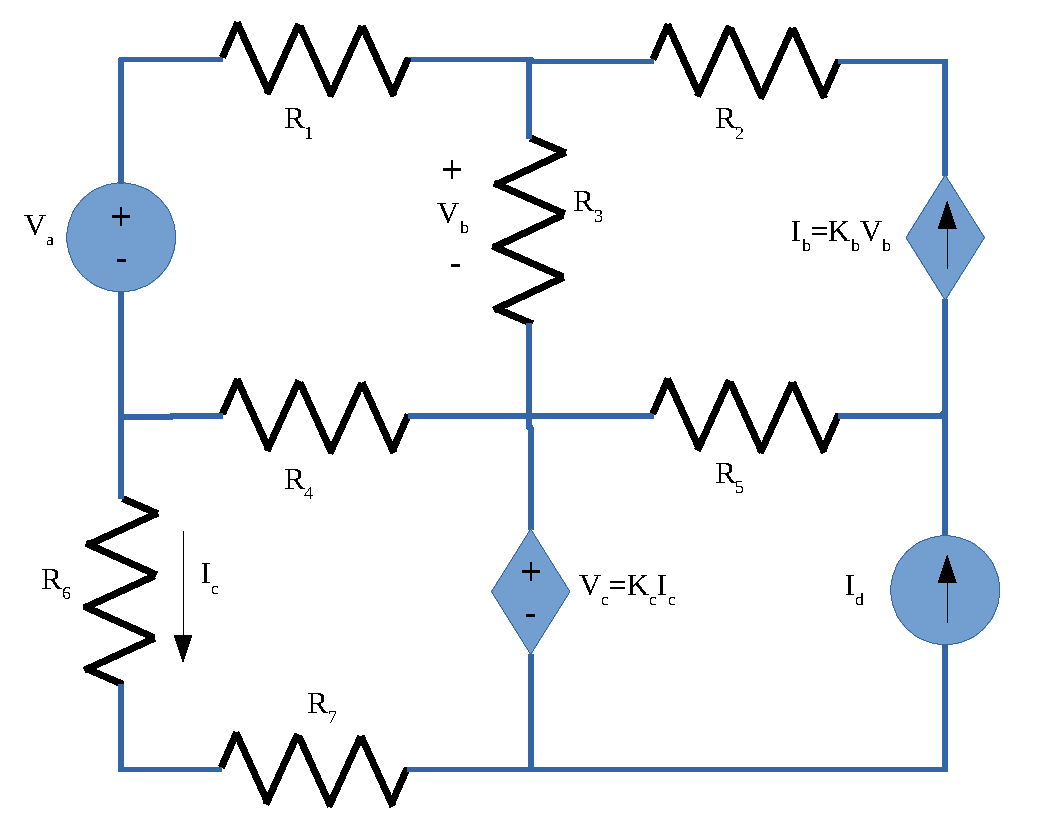
\includegraphics[width=0.8\linewidth]{circuit.pdf}
\caption{Circuit topography}
\label{fig:circuit}
\end{figure}

\begin{table}[H]
  \centering
  \begin{tabular}{|l|r|}
    \hline    
    {\bf Name} & {\bf Value} \\ \hline
    $R_1$ & 1k Ohm \\ \hline
    $R_2$ & 1k Ohm \\ \hline
    $R_3$ & 100k Ohm \\ \hline
    $R_4$ & 10k Ohm \\ \hline
    $R_5$ & 10k Ohm \\ \hline
    $R_6$ & 10k Ohm \\ \hline	
    $R_7$ & 1k Ohm \\ \hline	
    $C_1$ & 220n F \\ \hline
    $C_2$ & 220n F \\ \hline
    $C_3$ & 220n F \\ \hline	
  \end{tabular}
  \caption{Resistor and Capacitor values used in the circuit.}
  \label{tab:values}
\end{table}

\begin{equation}
	Merit = \frac{1}{Cost+Frequency Deviation + Gain Deviation + 10^{-6}}
\label{eq:merit}
\end{equation}

\newpage

\section{Theoretical analysis}

\label{sec:analysis}

\tab In this section, the circuit shown in Figure~\ref{fig:circuit} is analysed theoretically.

This circuit consists of an AMP-OP 741 and several resistances and capacitors. To analyse this circuit we considered the AMP-OP to be ideal (Zi = infinite and Zo = 0) and then we used nodal and mesh methods to derive the following equations:

\begin{equation}
\left|Z_{i}\right|=\left|Z_{C 1}+R 1 / / \infty\right|=\left|Z_{C 1}+R 1\right|
\end{equation}

\begin{equation}
\left|Z_{o}\right|=\left|Z_{C 2} / /(R 2+R 3 / / 0)\right|=\left|Z_{C 2} / / R 2\right|
\end{equation}

\begin{equation}
\left\{\begin{array}{l}
v_{-}=v_{+}=\frac{R 1}{R 1+Z_{C 1}} v_{i} \\
v_{A}=\left(1+\frac{R 3}{R 4}\right) v_{-} \\
v_{o}=\frac{Z_{C 2}}{Z_{C 2}+R 2} v_{A}
\end{array}\right.
\end{equation}

To obtain the central frequency, we calculated the average between the High Cut-off frequency (wh) and the Low Cut-off frequency (wl):
\begin{equation}
\omega_{0}=\sqrt{\omega_{L} * \omega_{H}}
\end{equation}

With these parameters we we're able to obtain a bandpass filter and by solving the previously presented equations we reached the following characteristics and frequency response graphic for the filter:


\begin{figure}[H] \centering
    \includegraphics[width=0.5\linewidth]{theo.eps}
    \caption{Theoretical frequency response.}
    \label{fig:theo1}
\end{figure}

\begin{table}[H]
    \centering
    \begin{tabular}{|l|r|}
    \hline
    {\bf Name} & {\bf Value} \\ \hline
   \input{../mat/gain.tex}
    \end{tabular}
    \caption{Voltage gain, bandwidth, central frequency, frequency and gain devitions.}
    \label{tab:theo1}
\end{table}


\begin{table}[H]
    \centering
    \begin{tabular}{|l|r|}
    \hline
    {\bf Name} & {\bf Value} \\ \hline
   \input{../mat/imp_octave.tex}
    \end{tabular}
    \caption{Absolute values for input and output impedances.}
    \label{tab:theo2}
\end{table}
%tabela
%grafico

\newpage

\section{Simulation Analysis}
\label{sec:simulation}

\subsection{Operating Point Analysis}

Table~\ref{tab:op} shows the simulated operating point results for the circuit
under analysis. Compared to the theoretical analysis results, one notices the
following differences: describe and explain the differences.

\begin{table}[h]
  \centering
  \begin{tabular}{|l|r|}
    \hline    
    {\bf Name} & {\bf Value [A or V]} \\ \hline
    @cb[i] & 0.000000e+00\\ \hline
@ce[i] & 0.000000e+00\\ \hline
@q1[ib] & 7.022567e-05\\ \hline
@q1[ic] & 1.404513e-02\\ \hline
@q1[ie] & -1.41154e-02\\ \hline
@q1[is] & 5.765392e-12\\ \hline
@rc[i] & 1.411536e-02\\ \hline
@re[i] & 1.411536e-02\\ \hline
@rf[i] & 7.022567e-05\\ \hline
@rs[i] & 0.000000e+00\\ \hline
v(1) & 0.000000e+00\\ \hline
v(2) & 0.000000e+00\\ \hline
base & 2.254108e+00\\ \hline
coll & 5.765392e+00\\ \hline
emit & 1.411536e+00\\ \hline
vcc & 1.000000e+01\\ \hline

  \end{tabular}
  \caption{Operating point. A variable preceded by @ is of type {\em current}
    and expressed in Ampere; other variables are of type {\it voltage} and expressed in
    Volt.}
  \label{tab:op}
\end{table}

\lipsum[1-1]


\subsection{Transient Analysis}

Figure~\ref{fig:trans} shows the simulated transient analysis results for the
circuit under analysis. Compared to the theoretical analysis results, one
notices the following differences: describe and explain the differences.

\begin{figure}[h] \centering
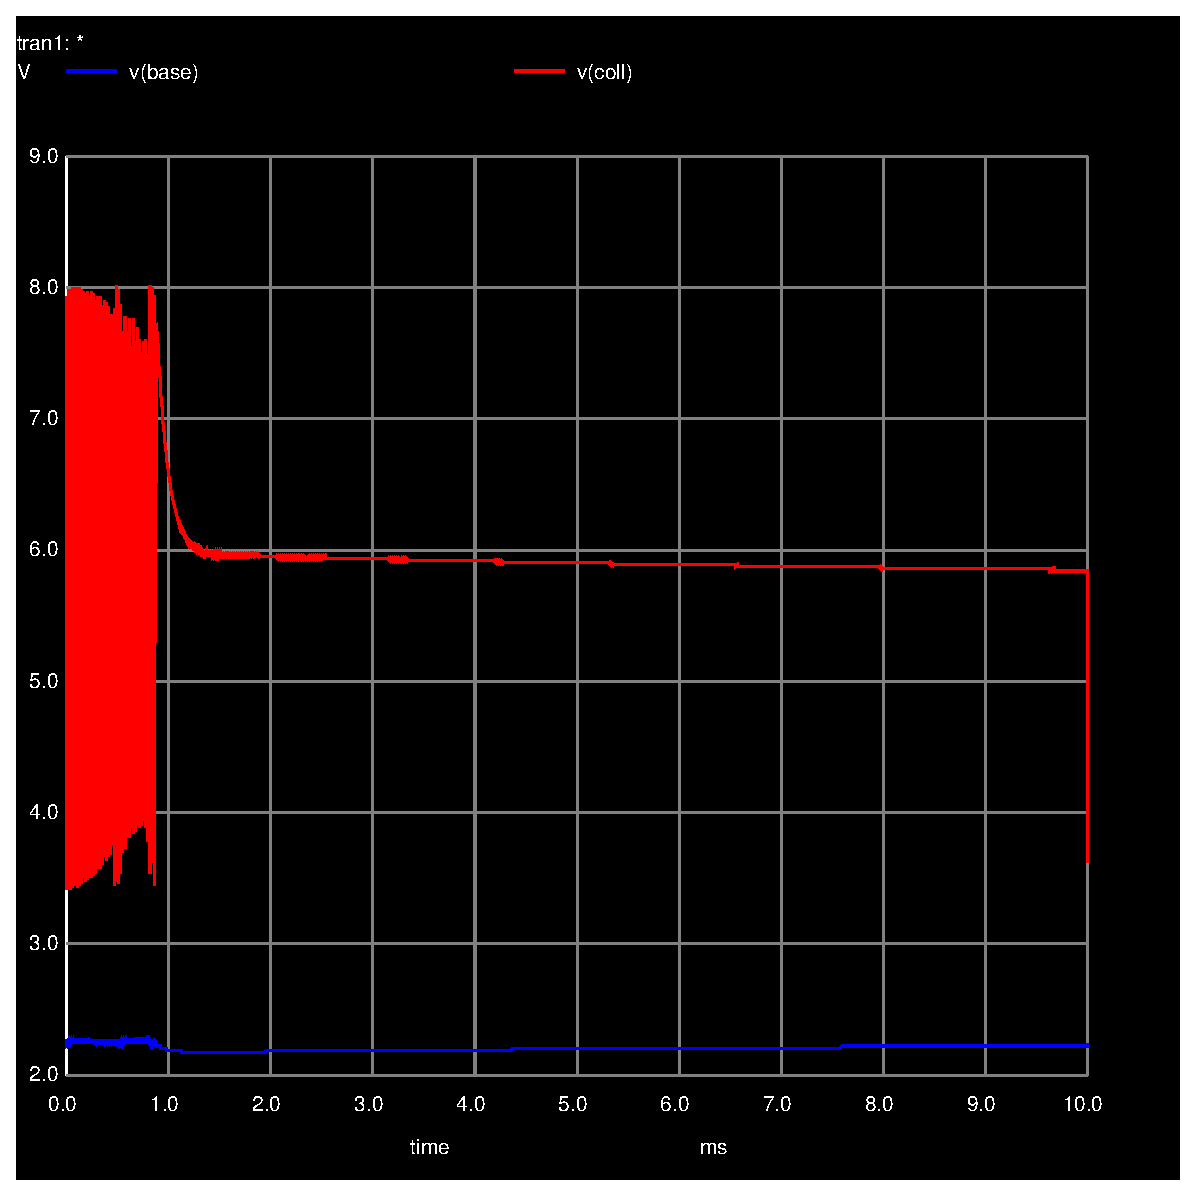
\includegraphics[width=0.6\linewidth]{trans.eps}
\caption{Transient output voltage}
\label{fig:trans}
\end{figure}

\lipsum[1-1]



\subsection{Frequency Analysis}

\subsubsection{Magnitude Response}

Figure~\ref{fig:acm} shows the magnitude of the frequency response for the
circuit under analysis. Compared to the theoretical analysis results, one
notices the following differences: describe and explain the differences.

\begin{figure}[h] \centering
\includegraphics[width=0.6\linewidth]{acm.eps}
\caption{Magnitude response}
\label{fig:acm}
\end{figure}

\lipsum[1-1]

\subsubsection{Phase Response}

Figure~\ref{fig:acp} shows the magnitude of the frequency response for the
circuit under analysis. Compared to the theoretical analysis results, one
notices the following differences: describe and explain the differences.

\begin{figure}[h] \centering
\includegraphics[width=0.6\linewidth]{acp.eps}
\caption{Phase response}
\label{fig:acp}
\end{figure}

\lipsum[1-1]

\subsubsection{Input Impedance}

Figure~\ref{fig:zim} shows the magnitude of the frequency response for the
circuit under analysis. Compared to the theoretical analysis results, one
notices the following differences: describe and explain the differences.

\begin{figure}[h] \centering
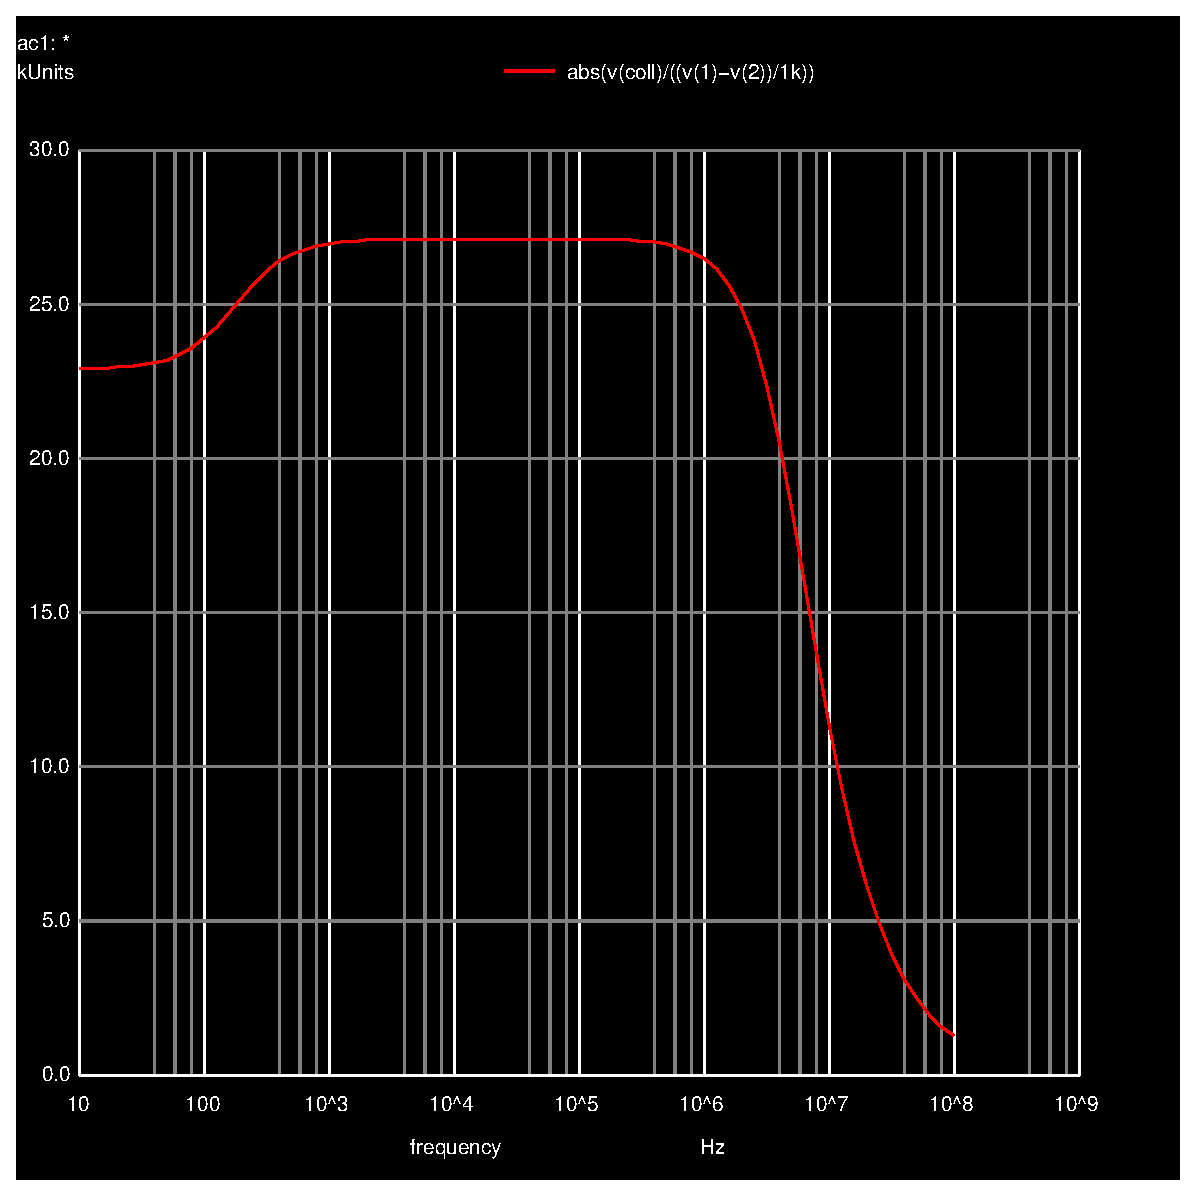
\includegraphics[width=0.6\linewidth]{zim.eps}
\caption{Input impedance}
\label{fig:zim}
\end{figure}

\lipsum[1-1]




\newpage

\section{Conclusion}
\label{sec:conclusion}

\tab The objective of this laboratory assignment as been accomplished as can be seen by the results obtained. The Ngspice simulator is a very powerful tool, as we can see by aproximating very acurately the theorical model.\par
As can be seen by comparing the tables and figures, both Octave maths tool and circuit simulator Ngspice data match, almost perfectly, the differences are explained by the rounding of the last decimal case. Once again, the model used can be seen to accurately describe the results we obtain, as it was to be expected.

%\cleardoublepage

% ----------------------------------------------------------------------
%  Bibliography
% ----------------------------------------------------------------------
%\addcontentsline{toc}{section}{\bibname}
%\bibliographystyle{abbrvunsrtnat} % <<<<< SELECT IF USING REFERENCES BY NUMBER (CITATION ORDER)
%\bibliography{../../../BIBfile.bib}

% ----------------------------------------------------------------------
\end{document}
% ----------------------------------------------------------------------

